\documentclass[]{article}
\usepackage{lmodern}
\usepackage{amssymb,amsmath}
\usepackage{ifxetex,ifluatex}
\usepackage{fixltx2e} % provides \textsubscript
\ifnum 0\ifxetex 1\fi\ifluatex 1\fi=0 % if pdftex
  \usepackage[T1]{fontenc}
  \usepackage[utf8]{inputenc}
\else % if luatex or xelatex
  \ifxetex
    \usepackage{mathspec}
  \else
    \usepackage{fontspec}
  \fi
  \defaultfontfeatures{Ligatures=TeX,Scale=MatchLowercase}
\fi
% use upquote if available, for straight quotes in verbatim environments
\IfFileExists{upquote.sty}{\usepackage{upquote}}{}
% use microtype if available
\IfFileExists{microtype.sty}{%
\usepackage{microtype}
\UseMicrotypeSet[protrusion]{basicmath} % disable protrusion for tt fonts
}{}
\usepackage[margin=1in]{geometry}
\usepackage{hyperref}
\hypersetup{unicode=true,
            pdftitle={faoswsStandardization: pullDataToSUA plugin},
            pdfauthor={Cristina Muschitiello Food and Agriculture Organization of the United Nations},
            pdfborder={0 0 0},
            breaklinks=true}
\urlstyle{same}  % don't use monospace font for urls
\usepackage{graphicx,grffile}
\makeatletter
\def\maxwidth{\ifdim\Gin@nat@width>\linewidth\linewidth\else\Gin@nat@width\fi}
\def\maxheight{\ifdim\Gin@nat@height>\textheight\textheight\else\Gin@nat@height\fi}
\makeatother
% Scale images if necessary, so that they will not overflow the page
% margins by default, and it is still possible to overwrite the defaults
% using explicit options in \includegraphics[width, height, ...]{}
\setkeys{Gin}{width=\maxwidth,height=\maxheight,keepaspectratio}
\IfFileExists{parskip.sty}{%
\usepackage{parskip}
}{% else
\setlength{\parindent}{0pt}
\setlength{\parskip}{6pt plus 2pt minus 1pt}
}
\setlength{\emergencystretch}{3em}  % prevent overfull lines
\providecommand{\tightlist}{%
  \setlength{\itemsep}{0pt}\setlength{\parskip}{0pt}}
\setcounter{secnumdepth}{5}
% Redefines (sub)paragraphs to behave more like sections
\ifx\paragraph\undefined\else
\let\oldparagraph\paragraph
\renewcommand{\paragraph}[1]{\oldparagraph{#1}\mbox{}}
\fi
\ifx\subparagraph\undefined\else
\let\oldsubparagraph\subparagraph
\renewcommand{\subparagraph}[1]{\oldsubparagraph{#1}\mbox{}}
\fi

%%% Use protect on footnotes to avoid problems with footnotes in titles
\let\rmarkdownfootnote\footnote%
\def\footnote{\protect\rmarkdownfootnote}

%%% Change title format to be more compact
\usepackage{titling}

% Create subtitle command for use in maketitle
\newcommand{\subtitle}[1]{
  \posttitle{
    \begin{center}\large#1\end{center}
    }
}

\setlength{\droptitle}{-2em}
  \title{faoswsStandardization:\\
\texttt{pullDataToSUA} plugin}
  \pretitle{\vspace{\droptitle}\centering\huge}
  \posttitle{\par}
  \author{Cristina Muschitiello\\
Food and Agriculture Organization of the United Nations}
  \preauthor{\centering\large\emph}
  \postauthor{\par}
  \predate{\centering\large\emph}
  \postdate{\par}
  \date{1 June 2018}

\usepackage{lscape}
\usepackage{booktabs}
\usepackage{longtable}
\usepackage{array}
\usepackage{multirow}
\usepackage[table]{xcolor}
\usepackage{wrapfig}
\usepackage{float}
\usepackage{colortbl}
\usepackage{pdflscape}
\usepackage{tabu}
\usepackage{threeparttable}
\usepackage{threeparttablex}
\usepackage[normalem]{ulem}
\usepackage{makecell}

\usepackage{draftwatermark}
\usepackage{makeidx}
\makeindex
\usepackage{float}
\floatplacement{figure}{H}
\usepackage{amsmath}
\usepackage{amssymb}
\usepackage{amsthm}
\usepackage{mathtools}
\usepackage{caption}

\begin{document}
\maketitle
\begin{abstract}
This vignette provides a description of the data Pulling Procedure: it
is the module that pull the data from different data-sets of different
domains, inside the table \texttt{sua\_unbalanced}, starting point of
the overall Standardization and Balancing procedure.
\end{abstract}

{
\setcounter{tocdepth}{4}
\tableofcontents
}
\newpage

\listoffigures

\subsection*{Disclaimer}\label{disclaimer}
\addcontentsline{toc}{subsection}{Disclaimer}

This Working Paper should not be reported as representing the official
view of the FAO. The views expressed in this Working Paper are those of
the author and do not necessarily represent those of the FAO or FAO
policy. Working Papers describe research in progress by the authors and
are published to elicit comments and to further discussion.

This paper is dynamically generated on \today{} and is subject to
changes and updates.

\newpage

\section*{The Data flow}\label{the-data-flow}
\addcontentsline{toc}{section}{The Data flow}

This is the first step of the Standardization and Balancing, the step in
which data coming from all output dataset are combined in another
dataset, which will be the starting point of the following step. It is
represented in figure \ref{fig:f1}

\begin{figure}[H]

{\centering 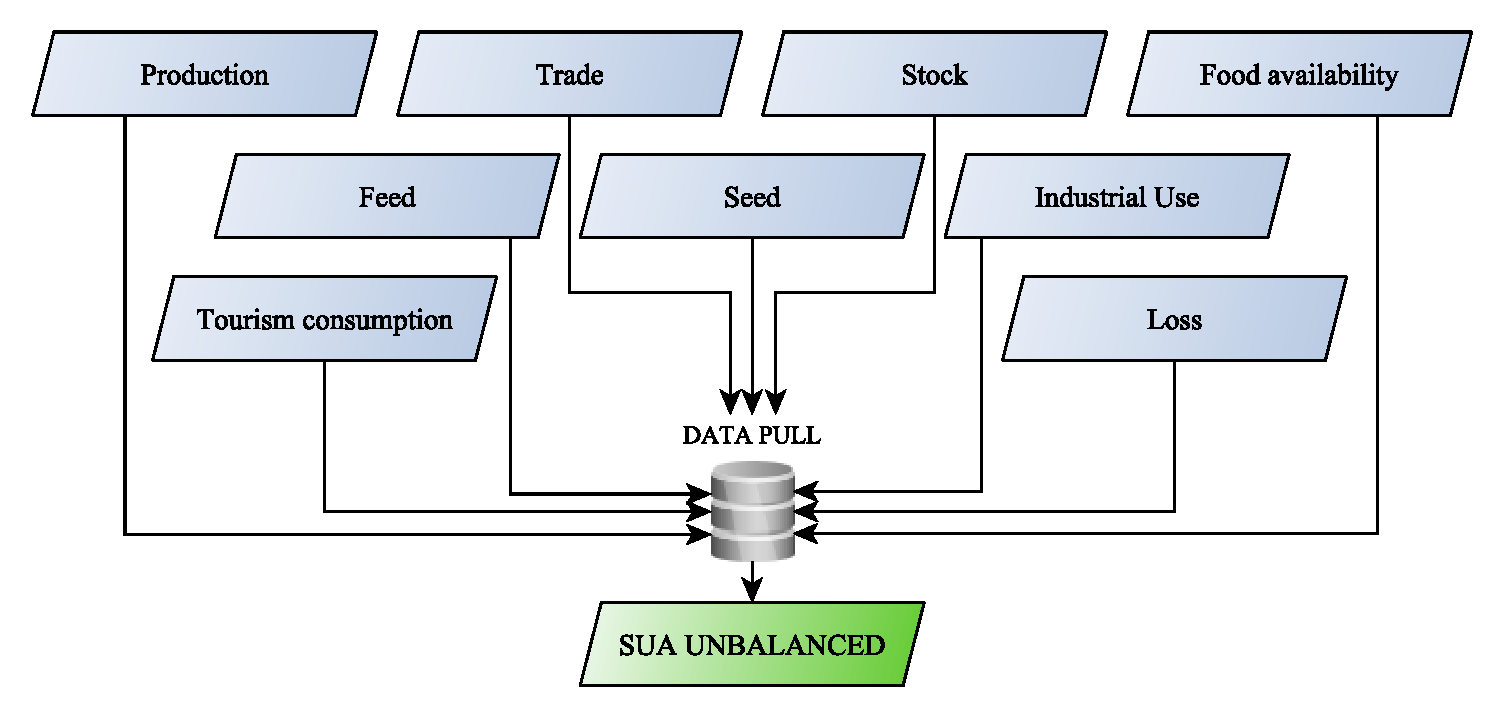
\includegraphics[width=1\linewidth]{images/pullData/01_pulldata} 

}

\caption{\label{fig:f1}Data pulling}\label{fig:f1}
\end{figure}

Notice that, from \emph{agriculture production} the following Data are
pulled:

\begin{itemize}
\tightlist
\item
  crop production,
\item
  livestok,
\item
  milk and eggs,
\item
  production of derived commodities,
\item
  seed,
\item
  feed.
\end{itemize}

\section*{Plug-in}\label{plug-in}
\addcontentsline{toc}{section}{Plug-in}

A general descriprion of all the objects of the \emph{SWS} is given in
the document \emph{Food Balance Sheet workflow in the Statistical
Working System}. A plug-in, in this framework, is an executable process.
In this document, the steps for executing the \emph{pullDataToSUA}
plugin are explained:

\section{Log-in in the SWS}\label{log-in-in-the-sws}

\begin{figure}[H]

{\centering \includegraphics[width=1\linewidth]{images/pullData/02_swsLogin} 

}

\caption{\label{fig:f2}Log-in in the SWS}\label{fig:f2}
\end{figure}

\section{Open a new Session}\label{open-a-new-session}

\begin{figure}[H]

{\centering \includegraphics[width=1\linewidth]{images/pullData/03_NewSession2} 

}

\caption{\label{fig:f3}Open a new Session}\label{fig:f3}
\end{figure}

\section{Define dimendions of the
session}\label{define-dimendions-of-the-session}

For the Pulling of the data, a session has to be opened in the
\emph{target} dataset, which is the \emph{suafbs:sua\_unbalanced}.
Therefore \emph{SUA/FBS} domain and \emph{sua\_unbalanced} have to be
selected from the screen:

\begin{figure}[H]

{\centering \includegraphics[width=1\linewidth]{images/pullData/04_domain} 

}

\caption{\label{fig:f4}Select Domain}\label{fig:f4}
\end{figure}

\begin{figure}[H]

{\centering \includegraphics[width=1\linewidth]{images/pullData/05_dataset} 

}

\caption{\label{fig:f5}Select Dataset}\label{fig:f5}
\end{figure}

\newpage

\section{Make an run the query}\label{make-an-run-the-query}

The query has to be done only on the country for which the Pull data has
to be performed. Indeed the plugin could be performed on one of the two
following set of countries: \emph{session Countries} or \emph{all
countries}. In this example \emph{China, Mainland} is selected.

\begin{figure}[H]

{\centering \includegraphics[width=1\linewidth]{images/pullData/06_selectCountry} 

}

\caption{\label{fig:f6}Select Country/ies}\label{fig:f6}
\end{figure}

All elements here have to be seleted (figure \ref{fig:f7}) and all
items(\ref{fig:f8}). The years to be selected depend on the interest of
the user.

\begin{figure}[H]

{\centering \includegraphics[width=1\linewidth]{images/pullData/07_selectElement} 

}

\caption{\label{fig:f7}Select all Elements}\label{fig:f7}
\end{figure}

\begin{figure}[H]

{\centering \includegraphics[width=1\linewidth]{images/pullData/08_selectItemYear} 

}

\caption{\label{fig:f8}Select items and years}\label{fig:f8}
\end{figure}

When all Variables have been defined, the query can be run:

\begin{figure}[H]

{\centering \includegraphics[width=1\linewidth]{images/pullData/09_run} 

}

\caption{\label{fig:f9}Run query}\label{fig:f9}
\end{figure}

\begin{figure}[H]

{\centering \includegraphics[width=1\linewidth]{images/pullData/10_wait} 

}

\caption{\label{fig:f10}Execution run}\label{fig:f10}
\end{figure}

\section{The session}\label{the-session}

The new swssion is reported in figure \ref{fig:f11}. Items are in the
``codelis order'', which means in the way they are stored in the SWS.
This means that they have a numerical order but there might be some
codes in a position not consistent with their number, just because they
have been inserted in a different moment in the codelist.

\begin{figure}[H]

{\centering \includegraphics[width=1\linewidth]{images/pullData/11_session} 

}

\caption{\label{fig:f11}The new Session}\label{fig:f11}
\end{figure}

\emph{At the moment this dataset is filled with data coming from the old
system (dataset ``suaValidated2015''), from 2010 to 2013 for}
\textbf{\emph{all countries}}. On these set of data, some changes are
made from the users when the FBS are validated. If a data pull is
performed in this time range for these countries, the data taken from
old system would be overwritten. Is very important to look at the
hystory of data and ask for clarofocation to the las persons who saved
data.

\section{Open the plug-in window.}\label{open-the-plug-in-window.}

For run the plug-in first the window for the plug-in selection and
definition has to be opened (figure \ref{fig:f12}).

\begin{figure}[H]

{\centering \includegraphics[width=1\linewidth]{images/pullData/12_runPlugin} 

}

\caption{\label{fig:f12}Plug-in botton}\label{fig:f12}
\end{figure}

In the \texttt{script} session, select the plug-in
\emph{\texttt{pullDataToSUA}} (figures \ref{fig:f13} and \ref{fig:f14}).

\begin{figure}[H]

{\centering \includegraphics[width=1\linewidth]{images/pullData/13_pluginWindow} 

}

\caption{\label{fig:f13}Plug-in window}\label{fig:f13}
\end{figure}

\begin{figure}[H]

{\centering \includegraphics[width=1\linewidth]{images/pullData/14_selectPlugin} 

}

\caption{\label{fig:f14}Select Plug-in}\label{fig:f14}
\end{figure}

This will authomatically bring to a sub-window where the other variables
of this plugin can be selected (figure \ref{fig:f15}).

\begin{figure}[H]

{\centering \includegraphics[width=1\linewidth]{images/pullData/15_selectyearsCountries} 

}

\caption{\label{fig:f15}Select other parameters}\label{fig:f15}
\end{figure}

\begin{itemize}
\tightlist
\item
  \texttt{First\ Year}: the year from which data have to be pulled. As
  previously said, in this dataset there are Validated and old data up
  tp 2013, therefore in this example 2014 is selected as first year.
\item
  \texttt{Last\ Year}: the last year until which the data have to be
  pulled.
\item
  \texttt{countries\ to\ pull}: plugin could be run on ``session
  countries'' or ``all countries''. Time of execution has to be taken
  into account in this case. To run this plugin on all countries might
  require almost an hour and generate a session so big that the SWS is
  not able to handle it.
\end{itemize}

\section{Launch Plug-in.}\label{launch-plug-in.}

In the \emph{Execution mode} section of the window, the option
\emph{\texttt{Synchronous}} is selected as default. This option imply
that, when the \emph{\texttt{Launch\ R\ plugin}} button is clicked, the
run starts immediately. The other option, \emph{\texttt{Scheduled}},
imply that another window is opened for the selection of the time of
execution.

When the plug-in has finished to run, a window appears on the screen and
an email is sento to the user (figure \ref{fig:f18}).

\begin{figure}[H]

{\centering \includegraphics[width=1\linewidth]{images/pullData/16_launch} 

}

\caption{\label{fig:f16}Launch plug-in}\label{fig:f16}
\end{figure}

\begin{figure}[H]

{\centering \includegraphics[width=1\linewidth]{images/pullData/18_emailSent} 

}

\caption{\label{fig:f18}End of plug-in run}\label{fig:f18}
\end{figure}

\section{Session updated}\label{session-updated}

In the session, all the figure that have been changed/added from the
plug-in have a small red triangle on the top-left side of the figure box
(figure \ref{fig:f19}).

\begin{figure}[H]

{\centering \includegraphics[width=1\linewidth]{images/pullData/19_updatedFigures} 

}

\caption{\label{fig:f19}Updated session}\label{fig:f19}
\end{figure}

\section{Save back to the database}\label{save-back-to-the-database}

For the new figures to be used in following steps, the data have to be
saved to the database.

\begin{figure}[H]

{\centering \includegraphics[width=1\linewidth]{images/pullData/20_saveToDatabase} 

}

\caption{\label{fig:f20}Save to Database}\label{fig:f20}
\end{figure}


\end{document}
